\documentclass[a4]{article}
\usepackage{geometry}
\geometry{verbose,tmargin=2.5cm,bmargin=2.5cm,lmargin=3cm,rmargin=3cm}
\usepackage{amsmath,amssymb,amsthm}
\usepackage{graphicx}
\usepackage[utf8]{inputenc}
\usepackage{fancyvrb}
\usepackage{hyperref}
\usepackage{lscape}
\usepackage{adjustbox}
\usepackage{verbatim}
\usepackage{subcaption}
\usepackage{placeins}
\usepackage{array}
\usepackage{multirow}
\usepackage{makecell}

\title{ONELAB monopile pre-processor interface}
\author{\'A.G. Vega-Artiles}
\date{June 2023}

\begin{document}

\maketitle

\tableofcontents

\section{How to use}

\subsection{Introduction}

``ONELAB is an open-source, lightweight interface to finite element software. It is completely free: the default ONELAB software bundle contains the mesh generator Gmsh, the finite element solver GetDP and the optimization library conveks." \cite{onelabweb}.

\subsection{Problem description}

In this example, a ONELAB environment is developed by using the geometry for \textit{Tutorial 7a}. Figure \ref{fig:geometry} shows the geometry.\footnote{For more information see \textit{Tutorial 7a}.}

\begin{figure}[tbh!]
	\centering
	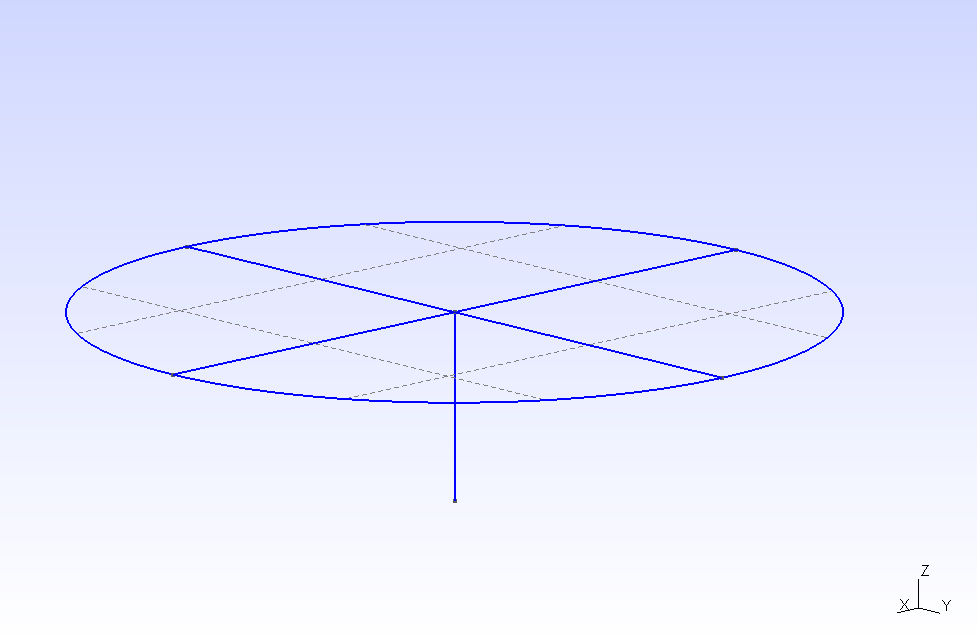
\includegraphics[scale=0.6]{geometry.png}
	\caption{Geometry.}
	\label{fig:geometry}
\end{figure}

\subsection{Procedure to setup the model}

The procedure followed to setup the model interactively consisted of the following steps:

\begin{itemize}

	\item The existing geometry file ``pile.geo" was loaded with ``File $\rightarrow$ Open".
	
	\item This file was merged with the file ``pile.pro" with ``File $\rightarrow$ Merge".
    
\end{itemize}

For more information about the procedure, examples and tutorials see \cite{onelabweb}. 

\subsection{Result}

The resulting ONELAB interface is shown in Figure \ref{fig:onelab_example}. The model is opened with the ONELAB software bundle by selecting the file ``pile.pro" with the Gmsh environment of the bundle. Everytime the file is opened all the parameters are reset, but can be modified interactively and a new mesh exported.

The interface has three additional parts in contrast to the regular Gmsh environment. These parts are:

\begin{itemize}
	\item \textbf{Geometry:} It is an additional Geometry menu related to the defined parameters (red square).
	
	\item \textbf{GetDP:} It is a menu related to the FEA. It is not used in this example (blue square).
	
	\item \textbf{Gmsh:} It shows the main files for the example (green square).
\end{itemize} 

\begin{figure}[tbh!]
	\centering
	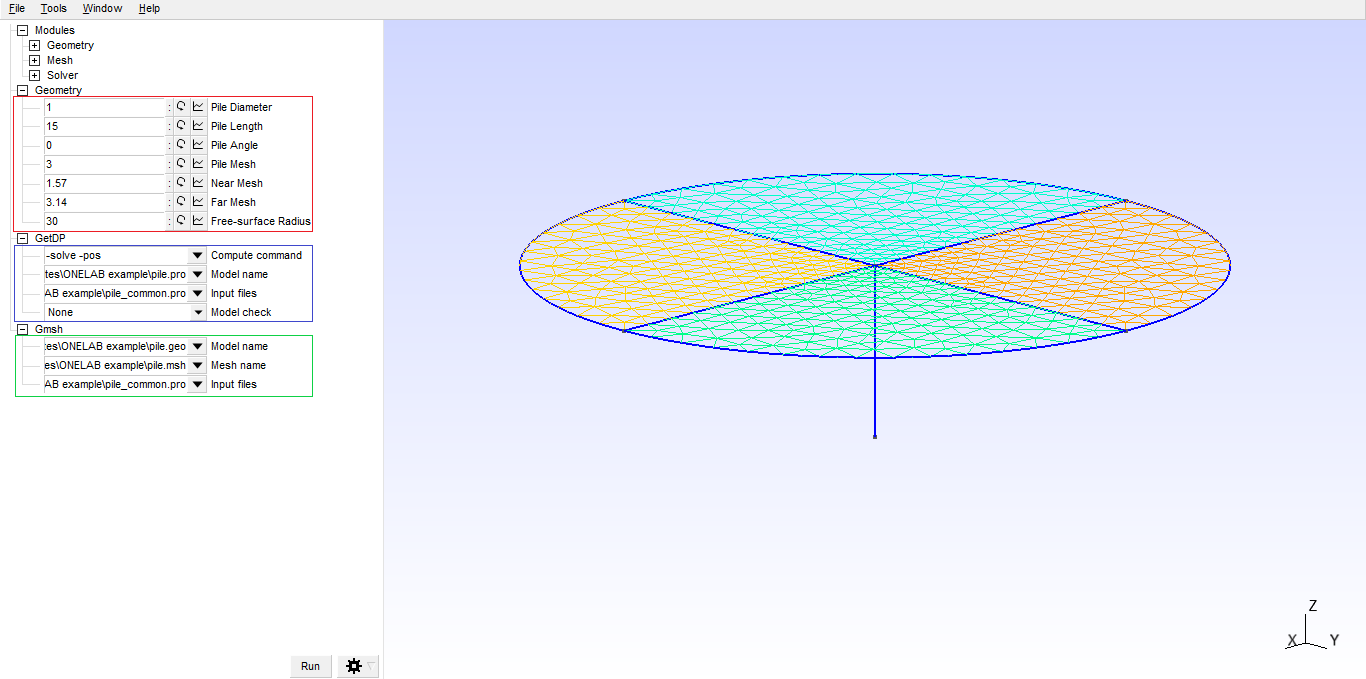
\includegraphics[scale=0.45]{onelab_example_coloured.png}
	\caption{ONELAB interface.}
	\label{fig:onelab_example}
\end{figure}

\section{Input files} 

\begin{itemize}
	\item \textbf{pile.geo:} This file defines the geometry of the problem and it is the same file used in \textit{Tutorial 7a}. The only difference with respect to the tutorial is that at the beginning of the file the variables are parametrized and the file ``pile\_common.pro" included. The change is the following:

\begin{Verbatim}	
Include "pile_common.pro";

// Geometry & mesh parameters
D = Diameter;
L = PL;
theta = TL;
ms_pile = PM;
ms_near = NM;
ms_far = FM;
R_truncation = Radius;

theta = TL*Pi/180;
\end{Verbatim}

	\item \textbf{pile\_common.pro:} This file is used to define the parameters that will appear in the graphical interface to be manipulated. They were previously set in the file ``pile.geo". These parameters are defined as numbers by means of the function ``DefineNumber" and every one has first the initial value to be shown, then its name with the format ``Geometry/Number + Name" that specifies its nature as geometric parameter and the position in the list for the graphical interface. Finally, same of them have the minimum and maximum values and the step between values to force to be integers. Furthermore, this file is included in the file ``pile.geo" to link both files. The script is the following:

\begin{Verbatim}
// Definition of parameters
Diameter = DefineNumber[1, Name "Geometry/1Pile Diameter", Min 1, Max 50, Step 1];
PL = DefineNumber[15, Name "Geometry/2Pile Length", Min 1, Max 50, Step 1];
TL = DefineNumber[0, Name "Geometry/3Pile Angle", Min -90, Max 90, Step 1];
PM = DefineNumber[3, Name "Geometry/4Pile Mesh"];
NM = DefineNumber[1.57, Name "Geometry/5Near Mesh"];
FM = DefineNumber[3.14, Name "Geometry/6Far Mesh"];
Radius = DefineNumber[30, Name "Geometry/7Free-surface Radius"];
\end{Verbatim}

	\item \textbf{pile.pro:} This file is the main file and is manly used to write the equations for the FEA, but, as this example is just made to manipulate the geometry of the problem, the only command in it is the inclusion of the file ``pile\_common.pro". The script is the following:

\begin{Verbatim}
Include "pile_common.pro";
\end{Verbatim}

\end{itemize}

For more information see \cite{onelabweb}. 

\FloatBarrier

\begin{thebibliography}{99}
		
	\bibitem{onelabweb} ``ONELAB". \url{https://onelab.info/}

\end{thebibliography}

\end{document}
